\section{Coevolution of heterogeneous multi-robot teams \cite{knudson2010coevolution}}

\begin{frame}{Problem Description}

\begin{figure}

\begin{columns}
\begin{column}{0.7\textwidth}
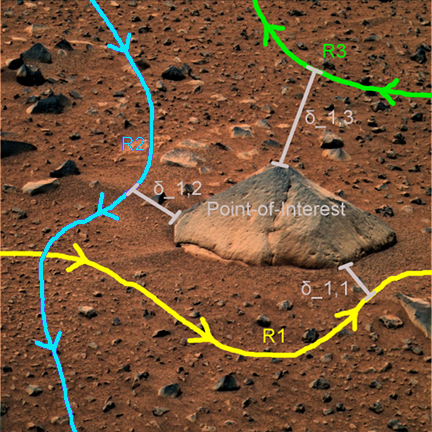
\includegraphics[width=\textwidth]{knudson-fig-2}
\end{column}
\begin{column}{0.3\textwidth}
\caption{
Figure 2 from \cite{knudson2010coevolution}.
}
\end{column}
\end{columns}
\end{figure}

\end{frame}

\begin{frame}

difference metric generalizes to other problem domains

however, with large groups and without shortcuts it could become computationally prohibitive

also, might break down for too much specialization
* analogy to curling sweepers vs throwers

\end{frame}
